% !TEX root = NSF_SuperCDMS_SNOLAB_OPS.tex
\section{Plan of Work}
\label{sec:planofwork}


The timing of the proposed work is driven by the proposed, yearly workshops that focus on (1) teaching scientists how to use the tools to access their data, (2) working with scientists to perform science analyses, (3) identifying usability improvements needed for the software, and (4) bringing developers into close contact with the science community using their tools.  Each workshop will result in an updated roadmap for the software.

Thus, the the primary milestones of the proposed work are (1) the workshops and the updated roadmap and (2) software releases that include testing, documentation, and example analyses.

The work for each yearly cycle can be broken down into the following categories: development of basic computing skills learning material; development of the data-access library; planning and execution of the workshop; and a community-driven update of the roadmap.  See Table~\ref{tab:WBS} for details on who will perform this work and Figure~\ref{fig:ops-schedule} for the yearly timeline.

The minimum requirements will determine the work plan each year; initial requirements are the following:

\begin{enumerate}
    \item If students or staff move on to other positions, their replacements should be able to get up to speed in a month or less.
    \item Someone with no domain knowledge but reasonable persistence should be able to run the example analysis within a week.
    \item Someone with no domain knowledge but reasonable persistence should be able to analyze their own data within a month.
    \item A scientist who uses the access-data library to obtain a science result should know how to cite the software.
    \item A scientist experiencing trouble using the software should be able to determine how to get help quickly (within five minutes of searching).
    \item A scientist who wishes to improve the code should be able to quickly determine how to contact the developers and how to change, test, and push the code.
\end{enumerate}

%The scope of the proposed software is relatively modest: copy an existing framework and adapt it so that it stores data in awkward-array structures rather than slower, dictionary structures.  The development and testing of this code will take time - but reference code for similar work exists, there is robust community support, and there is a developer guide that gives specific instructions for developers who wish to extend the existing Kaitai Struct code in this way.  The proposed work is feasible because it connects two libraries that are both designed for this purpose.

The majority of the proposed work is in making the modified software easy to use for scientists, and making it easy for the community to participate in the direction and development of the software.  This requires robust documentation for both users and developers.  Users will require installation instructions, instructions for using the library, and guidance on how to adapt the examples for their own analysis needs.  Developers will need additional documentation: instructions for changing the code and testing the code, and instructions and guidance on contributing their changes to the project.

%To meet the minimum requirements, the workplan involves creating of initial documentation and an automated testing suite by the Professional Research Associate and example analysis created by the Master's student.

%Undergraduates will begin either by working on new scientific computation skills or improving or adding to material of already-developed scientific computation skills.  Students who join the lab currently have two first projects to chose from: working through an introductory lab on water simulation, or working through an example analysis of gamma-spectroscopy data.  The students try to perform their work using existing documentation; the PI provides guidance when this is inadequate.  This provides an opportunity for students to design improvements and learn the basics of contributing to a code repository.  In addition to providing valuable training for the students, this process identifies gaps in the documentation that are often invisible to experts.

%This initial work is expected to result in improvements and additions to web-accessible tutorial materials.  In addition, this training will provide a foundation that will allow the students to attempt the following actions:
\begin{comment}
\begin{itemize}
    \item Successfully follow a simple example analysis using the data-access library.
    \item Successfully follow a tutorial to make and share a change to the library documentation.
    \item Successfully follow a tutorial to make, test, and share a change to the library source code.
\end{itemize}
\end{comment}

\begin{table}
\begin{tabularx}{\textwidth}{>{\hsize=1.5\hsize}X
                             >{\hsize=0.4\hsize}X
                             >{\hsize=0.4\hsize}X
                             >{\hsize=0.4\hsize}X
                             >{\hsize=0.5\hsize}X}
\toprule
                             Work & PI & PRA & Master's student & Undergrads\\
\midrule
%\rowcolor{gray!90}
Roadmap \& workplan development
& X & X & X & \\

Basic skills documentation 
& & & & X\\
\addlinespace[2mm]

\textit{Data-access library development}
& \\
\midrule
Code Development 
& & X & &\\

Code Documentation (this includes automated testing and contribution guidelines and instructions)
& & X & &\\

Example Analyses (will initially include XIA and SuperCDMS analysis)
& & & X &\\

User Testing (may feed back into basic skill documentation)
& & & X & X\\
\addlinespace[2mm]

\textit{Workshop}
& \\
\midrule
Recruiting
& X & & &\\
Organization
& & X & & X\\
Pre-workshop analysis coordination
& X & X & X & \\

%Community-driven update of roadmap
%& X & X & & \\
\bottomrule
\end{tabularx}
\caption{Primary work assignments for given tasks.  Community efforts are not listed here but will be encouraged wherever possible.}
\label{tab:WBS}
\end{table}

\begin{figure}[htb]
    \begin{center}
      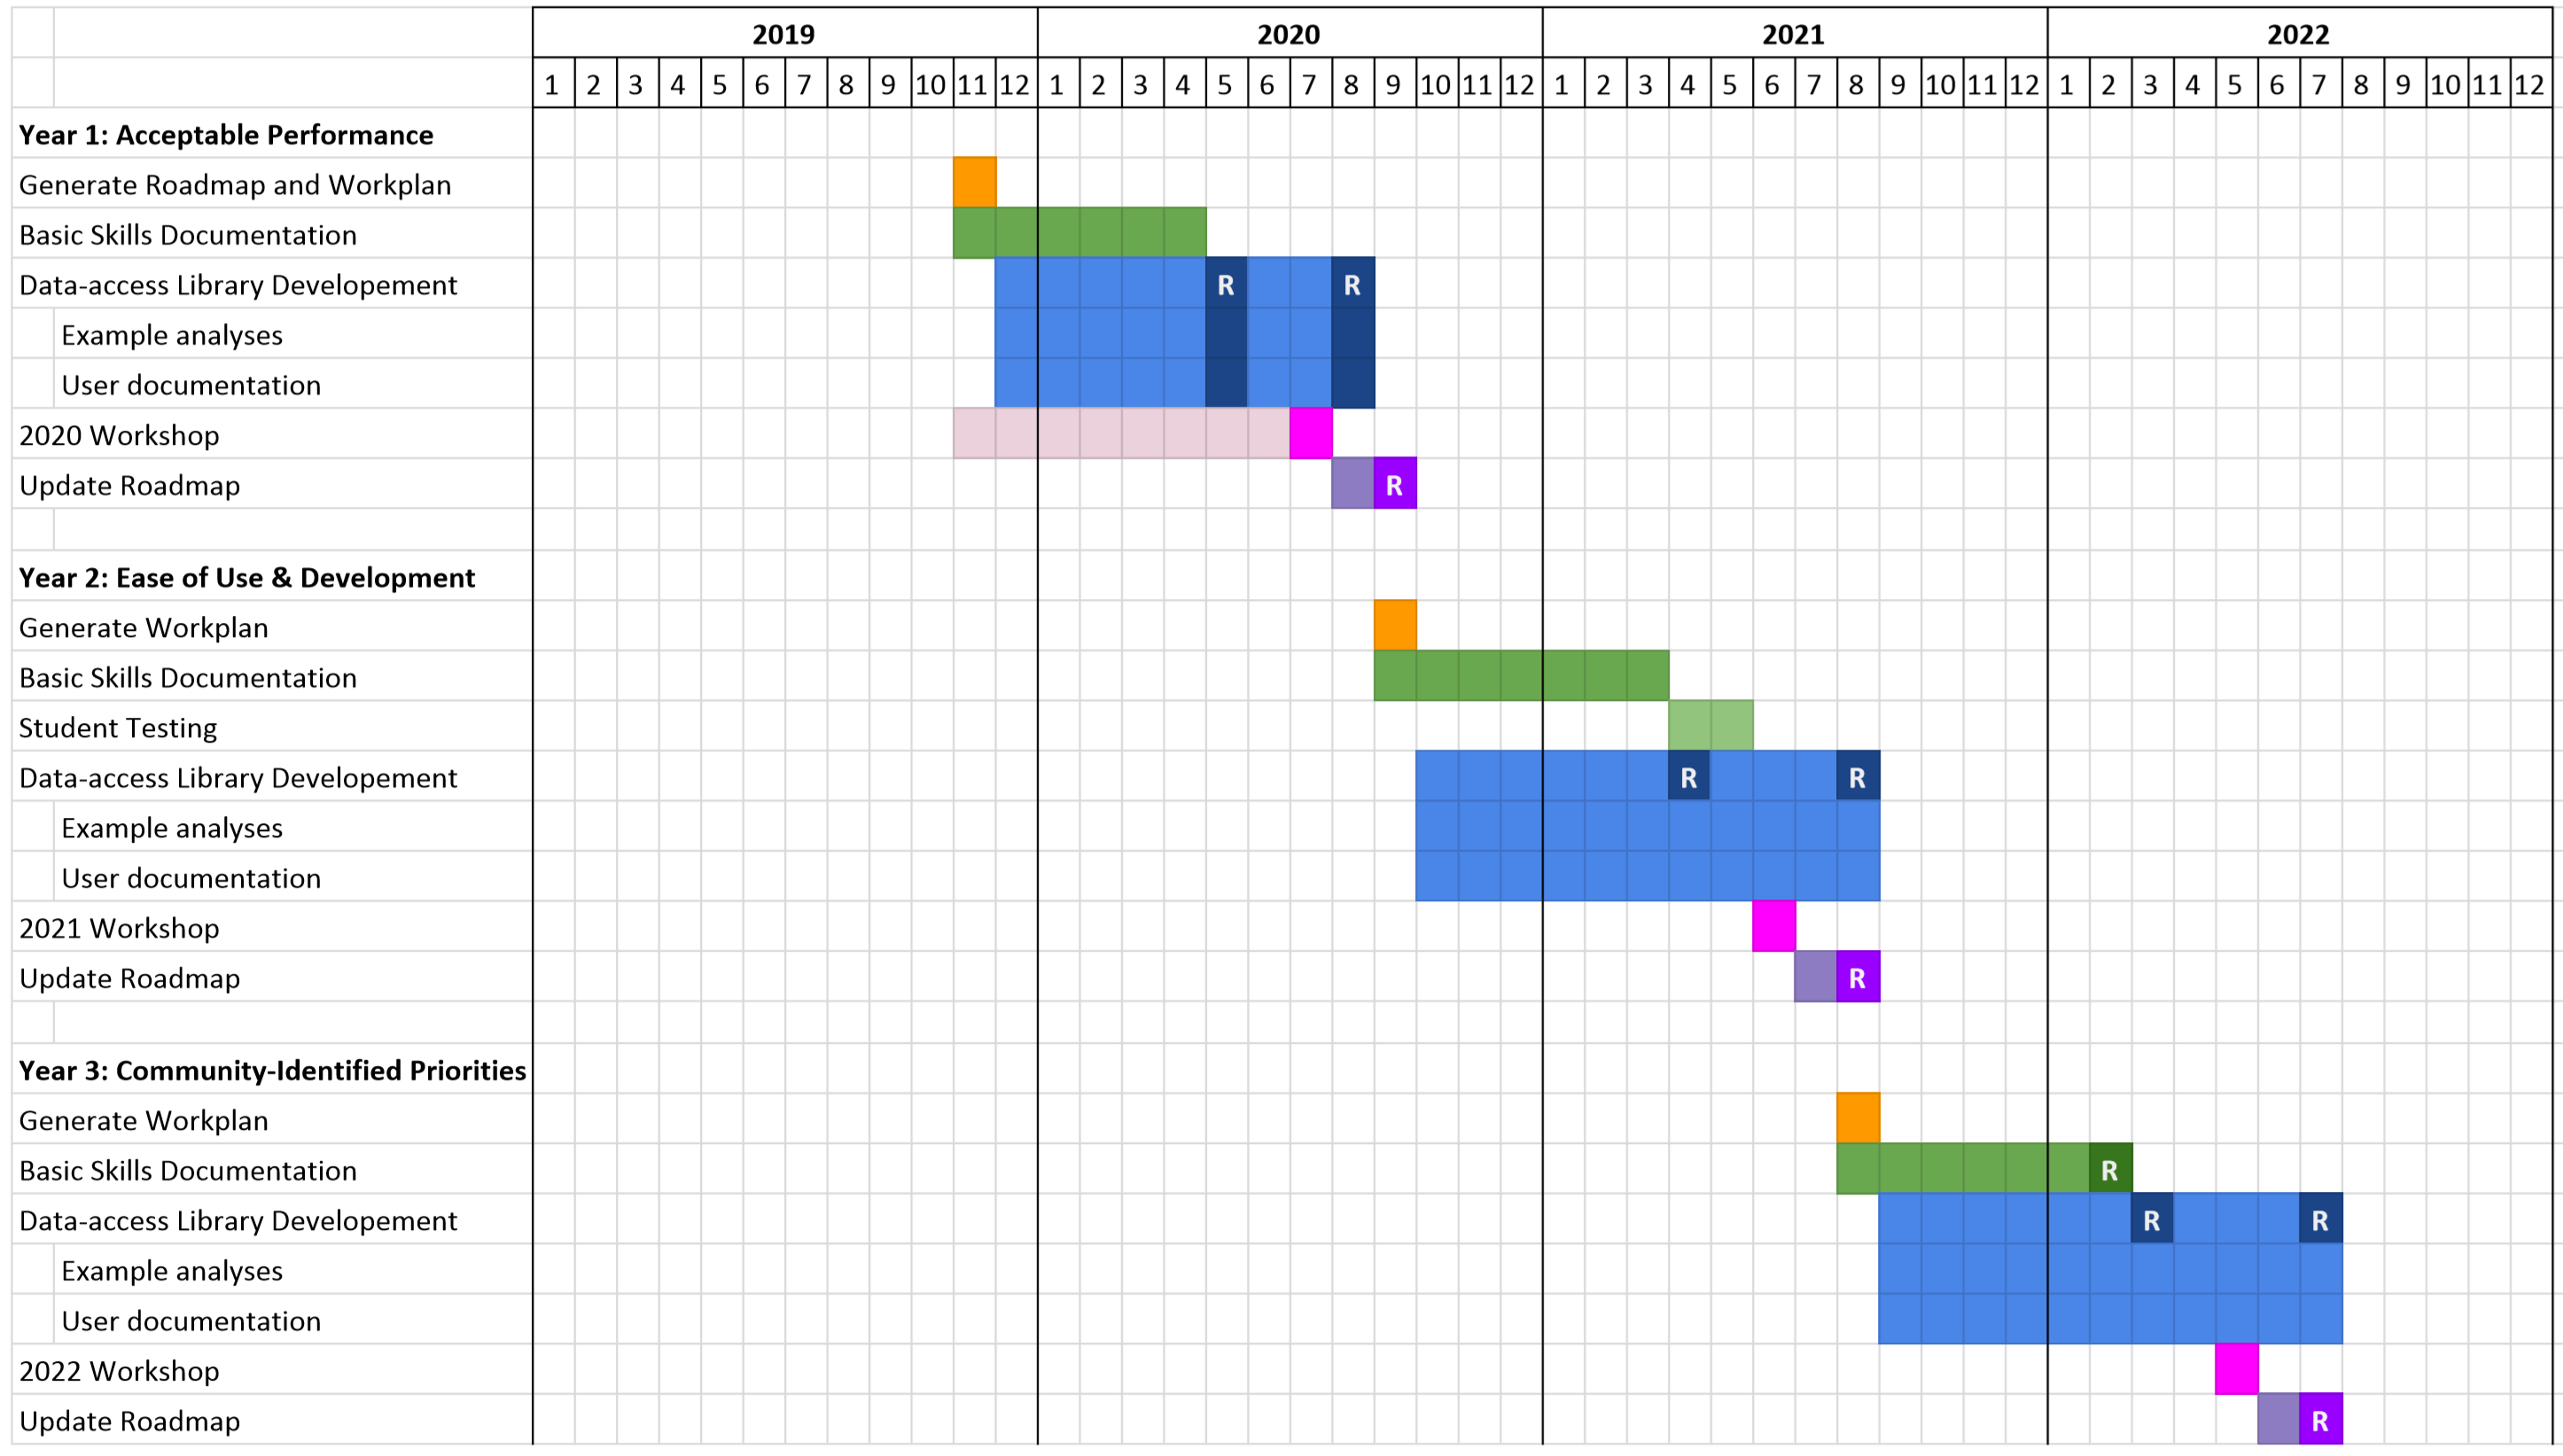
\includegraphics[width=\textwidth]{Figures/schedule2}
    \end{center}
    \caption{A schedule for the proposed work.  The yearly cycle: development and testing,  release and testing, and community workshop intends to build community involvement starting in year 1. Student testing is expected to be more intensive in years 2 and 3, when the documentation is better-developed.  Milestone releases are marked with ``R.''}
    \label{fig:ops-schedule}
\end{figure}